\section{Results}
\label{sec:results}

The final results of this analysis are displayed in Fig.~\ref{fig:results},
which shows the \lth parameters for the prompt and non-prompt \jpsi and \psip mesons,
with the vertical bars representing the statistical and systematic uncertainties 
summed in quadrature.

\begin{figure}[h]
\centering
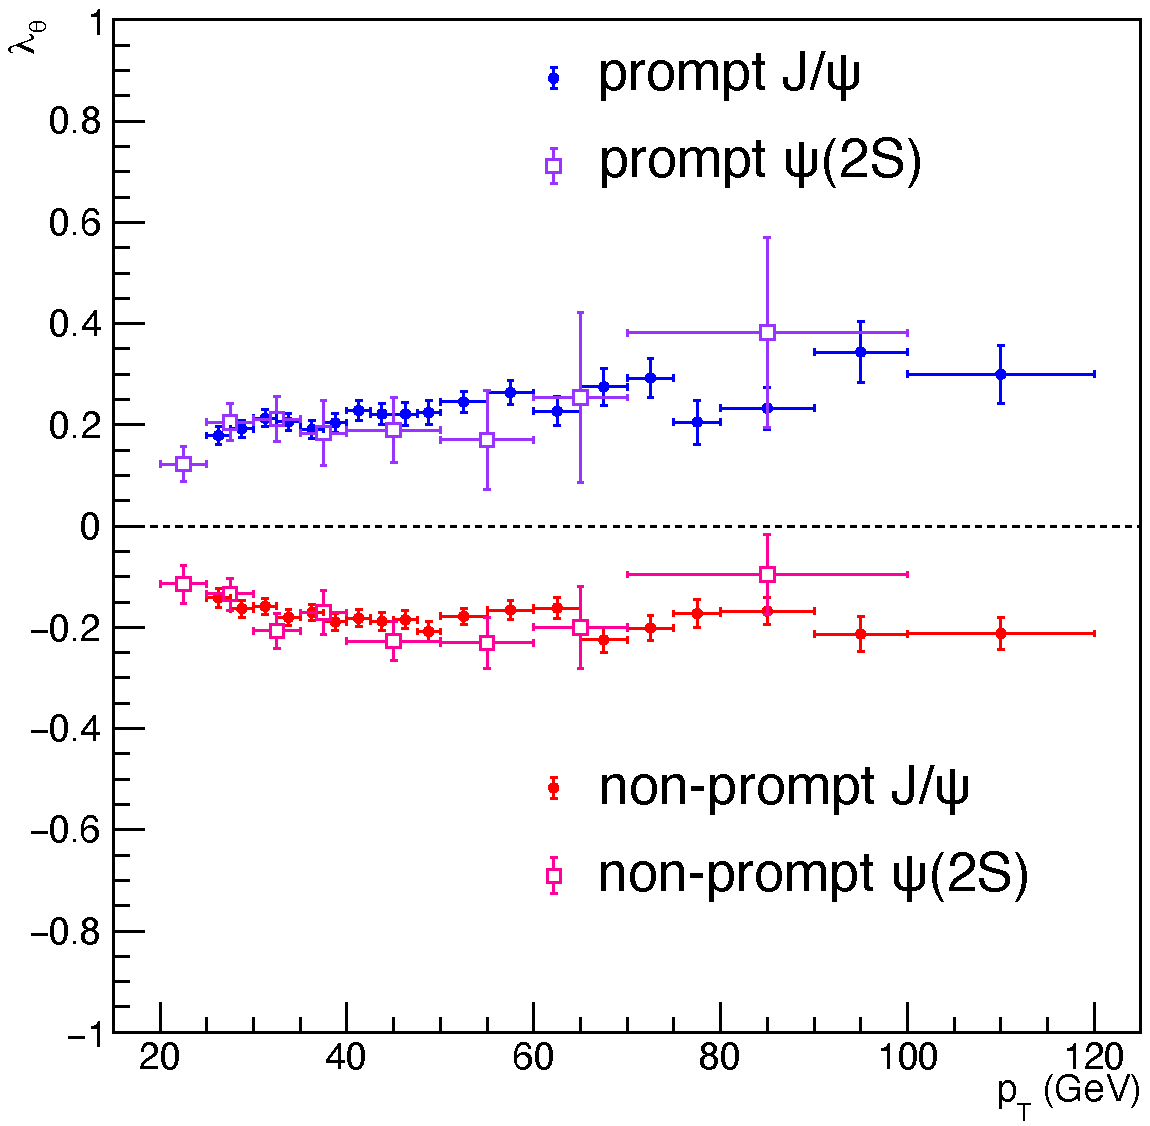
\includegraphics[width=0.65\textwidth]{Figures/chapter7/lth-PR-NP-jpsi-psip-final.pdf}
\caption{\lth parameter measured, as a function of \pt, 
for the prompt and non-prompt \jpsi and \psip mesons,
as indicated in the legends.
The vertical bars represent the statistical and systematic uncertainties 
summed in quadrature.}
\label{fig:results}
\end{figure}

The numerical values of these results are collected in 
Tables~\ref{tab:lth-jpsiPR}--\ref{tab:lth-psipNP}.

\begin{table}[h]
\centering 
\caption{\lth parameter measured in the HX frame, as a function of \pt, 
for the prompt \jpsi mesons.}
\label{tab:lth-jpsiPR}
% J/psi Prompt
\begin{tabular}{c|ccc}
\pt (GeV) & \lth & $\sigma_{\text{stat}}$ & $\sigma_{\text{sys}}$ \\
\hline
25--27.5 & $0.179$ & $\pm0.007$ & $\pm0.017$\\
27.5--30 & $0.192$ & $\pm0.008$ & $\pm0.015$\\
30--32.5 & $0.213$ & $\pm0.009$ & $\pm0.014$\\
32.5--35 & $0.206$ & $\pm0.010$ & $\pm0.013$\\
35--37.5 & $0.191$ & $\pm0.012$ & $\pm0.013$\\
37.5--40 & $0.204$ & $\pm0.013$ & $\pm0.013$\\
40--42.5 & $0.228$ & $\pm0.015$ & $\pm0.013$\\
42.5--45 & $0.221$ & $\pm0.017$ & $\pm0.012$\\
45--47.5 & $0.221$ & $\pm0.018$ & $\pm0.012$\\
47.5--50 & $0.224$ & $\pm0.021$ & $\pm0.012$\\
50--55 & $0.245$ & $\pm0.017$ & $\pm0.012$\\
55--60 & $0.264$ & $\pm0.021$ & $\pm0.012$\\
60--65 & $0.227$ & $\pm0.026$ & $\pm0.012$\\
65--70 & $0.275$ & $\pm0.034$ & $\pm0.012$\\
70--75 & $0.292$ & $\pm0.036$ & $\pm0.012$\\
75--80 & $0.205$ & $\pm0.042$ & $\pm0.012$\\
80--90 & $0.233$ & $\pm0.040$ & $\pm0.012$\\
90--100 & $0.344$ & $\pm0.059$ & $\pm0.012$\\
100--120 & $0.300$ & $\pm0.056$ & $\pm0.012$
\end{tabular}
\end{table}

\begin{table}[h]
\centering 
\caption{\lth parameter measured in the HX frame, as a function of \pt, 
for the non-prompt \jpsi mesons.}
\label{tab:lth-jpsiNP}
% J/psi Non-Prompt
\begin{tabular}{c|ccc}
\pt (GeV) & \lth & $\sigma_{\text{stat}}$ & $\sigma_{\text{sys}}$ \\
\hline
25--27.5 & $-0.141$ & $\pm0.007$ & $\pm0.017$\\
27.5--30 & $-0.163$ & $\pm0.007$ & $\pm0.015$\\
30--32.5 & $-0.158$ & $\pm0.008$ & $\pm0.014$\\
32.5--35 & $-0.180$ & $\pm0.008$ & $\pm0.013$\\
35--37.5 & $-0.170$ & $\pm0.009$ & $\pm0.013$\\
37.5--40 & $-0.189$ & $\pm0.010$ & $\pm0.013$\\
40--42.5 & $-0.182$ & $\pm0.011$ & $\pm0.013$\\
42.5--45 & $-0.188$ & $\pm0.012$ & $\pm0.012$\\
45--47.5 & $-0.185$ & $\pm0.013$ & $\pm0.012$\\
47.5--50 & $-0.208$ & $\pm0.015$ & $\pm0.012$\\
50--55 & $-0.178$ & $\pm0.011$ & $\pm0.012$\\
55--60 & $-0.166$ & $\pm0.014$ & $\pm0.012$\\
60--65 & $-0.162$ & $\pm0.017$ & $\pm0.012$\\
65--70 & $-0.225$ & $\pm0.021$ & $\pm0.012$\\
70--75 & $-0.201$ & $\pm0.021$ & $\pm0.012$\\
75--80 & $-0.173$ & $\pm0.026$ & $\pm0.012$\\
80--90 & $-0.168$ & $\pm0.023$ & $\pm0.012$\\
90--100 & $-0.213$ & $\pm0.032$ & $\pm0.012$\\
100--120 & $-0.212$ & $\pm0.030$ & $\pm0.012$
\end{tabular}
\end{table}

\begin{table}[h]
\centering 
\caption{\lth parameter measured in the HX frame, as a function of \pt, 
for the prompt \psip mesons.}
\label{tab:lth-psipPR}
% psi(2S) Prompt
\begin{tabular}{c|ccc}
\pt (GeV) & \lth & $\sigma_{\text{stat}}$ & $\sigma_{\text{sys}}$ \\
\hline
20--25 & $0.123$ & $\pm0.028$ & $\pm0.021$\\
25--30 & $0.205$ & $\pm0.033$ & $\pm0.016$\\
30--35 & $0.211$ & $\pm0.043$ & $\pm0.013$\\
35--40 & $0.184$ & $\pm0.063$ & $\pm0.012$\\
40--50 & $0.190$ & $\pm0.063$ & $\pm0.012$\\
50--60 & $0.170$ & $\pm0.098$ & $\pm0.012$\\
60--70 & $0.254$ & $\pm0.167$ & $\pm0.012$\\
70--100 & $0.382$ & $\pm0.187$ & $\pm0.012$
\end{tabular}
\end{table}

\begin{table}[h]
\centering 
\caption{\lth parameter measured in the HX frame, as a function of \pt, 
for the non-prompt \psip mesons.}
\label{tab:lth-psipNP}
% psi(2S) Non-Prompt
\begin{tabular}{c|ccc}
\pt (GeV) & \lth & $\sigma_{\text{stat}}$ & $\sigma_{\text{sys}}$ \\
\hline
20--25 & $-0.114$ & $\pm0.031$ & $\pm0.023$\\
25--30 & $-0.134$ & $\pm0.028$ & $\pm0.016$\\
30--35 & $-0.207$ & $\pm0.031$ & $\pm0.014$\\
35--40 & $-0.170$ & $\pm0.042$ & $\pm0.012$\\
40--50 & $-0.227$ & $\pm0.037$ & $\pm0.012$\\
50--60 & $-0.231$ & $\pm0.050$ & $\pm0.012$\\
60--70 & $-0.200$ & $\pm0.081$ & $\pm0.012$\\
70--100 & $-0.096$ & $\pm0.078$ & $\pm0.012$
\end{tabular}
\end{table}

